\chapter{Task 3}
\begin{parlist}
\item Assume that only correct values are given, e.g values in the correct range for the tests. A.points are the points from the first test, B.points are the points from the second test.
equivalence classes:
\begin{itemize}
\item Class A :  A.points + B.points >= 90 
\item Class B :  A.points + B.points > 75  and  A.points + B.points < 90 and A.points > 20 and B.points > 20
\item Class C:  A.points + B.points > 60  and  A.points + B.points <= 75 and A.points > 20 and B.points > 20
\item Class D:  A.points >= 20 and B.points >= 20  and  A.points + B.points <= 60 and A.points > 20 and B.points > 20
\item Class F:  A.points < 20 or B.points < 20
\end{itemize}
\item 
Class A:
\begin{lstlisting}[language=java,frame=trBL]
@Test
public void testA(){
   assertEquals("Pruefe Klasse A", Grader.Grade.A, Grader.grade(60,40));
}
\end{lstlisting}
Class B:
\begin{lstlisting}[language=java,frame=trBL]
@Test
public void testB(){
   assertEquals("Pruefe Klasse B", Grader.Grade.B, Grader.grade(30,50));
}
\end{lstlisting}
Class C:
\begin{lstlisting}[language=java,frame=trBL]
@Test
public void testC(){
   assertEquals("Pruefe Klasse C",  Grader.Grade.C, Grader.grade(30,30));
}
\end{lstlisting}
Class D:
\begin{lstlisting}[language=java,frame=trBL]
@Test
public void testD(){
   assertEquals("Pruefe Klasse D",  Grader.Grade.D, Grader.grade(25,25));
}
\end{lstlisting}
Class F:
\begin{lstlisting}[language=java,frame=trBL]
@Test
public void testF(){
   assertEquals("Pruefe Klasse F",  Grader.Grade.F, Grader.grade(5,5));
}
\end{lstlisting}

\item Testcases for each of the boundary edges between the different equivalence classes.
\begin{lstlisting}[language=java,frame=trBL]
	@Test
	public void testFtoD1() {
		assertEquals("Pruefe Grenzuebergang F zu D Nr. 1", Grader.Grade.F, Grader.grade(30, 19));
	}

	@Test
	public void testDtoF1() {
		assertEquals("Pruefe Grenzuebergang D zu F Nr. 1", Grader.Grade.D, Grader.grade(30, 21));
	}

	@Test
	public void testFtoD2() {
		assertEquals("Pruefe Grenzuebergang F zu D Nr. 2", Grader.Grade.F, Grader.grade(19, 25));
	}

	@Test
	public void testDtoF2() {
		assertEquals("Pruefe Grenzuebergang D zu F Nr. 2", Grader.Grade.D, Grader.grade(21, 25));
	}

	@Test
	public void testDtoC() {
		assertEquals("Pruefe Grenzuebergang D zu C ", Grader.Grade.D, Grader.grade(30, 30));
		
	}
	
	@Test
	public void testCtoD() {
		assertEquals("Pruefe Grenzuebergang C zu D ", Grader.Grade.C, Grader.grade(31, 31));
	}

	@Test
	public void testFtoC() {
		assertEquals("Pruefe Grenzuebergang F zu C", Grader.Grade.F, Grader.grade(19, 45));
	}
	
	@Test
	public void testCtoF() {
		assertEquals("Pruefe Grenzuebergang C zu F", Grader.Grade.C, Grader.grade(20, 45));
	}

	@Test
	public void testCtoB() {
		assertEquals("Pruefe Grenzuebergang C zu B", Grader.Grade.C, Grader.grade(30, 44));
	}
	
	@Test
	public void testBtoC() {
		assertEquals("Pruefe Grenzuebergang B zu C", Grader.Grade.B, Grader.grade(30, 45));
	}

	@Test
	public void testFtoB() {
		assertEquals("Pruefe Grenzuebergang F zu B", Grader.Grade.F, Grader.grade(19, 55));
	}
	
	@Test
	public void testBtoF() {
		assertEquals("Pruefe Grenzuebergang B zu F", Grader.Grade.B, Grader.grade(20, 55));
	}

	@Test
	public void testBtoA() {
		assertEquals("Pruefe Grenzuebergang B zu A", Grader.Grade.B, Grader.grade(35, 54));
	}
	
	@Test
	public void testAtoB() {
		assertEquals("Pruefe Grenzuebergang A zu B", Grader.Grade.A, Grader.grade(35, 55));
	}

\end{lstlisting}

\center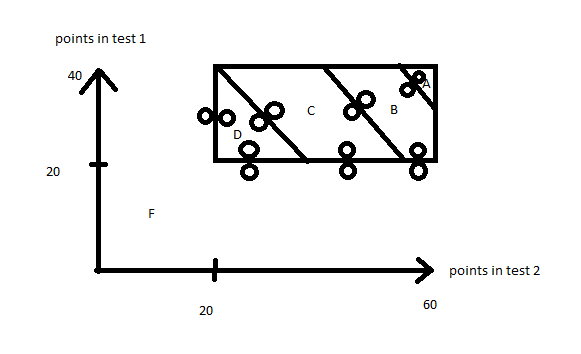
\includegraphics{Immagini/diagram.png}



\item (d) We detected following defects, the Grader.grade() method returns grade B for the input 35 55 which should be grade A because it 35+55 is 90. This is likely caused by the implementation using a ">" rather than a ">=" in the conditional statement. And Grader.grade() returns grade C for the input 30 30 which should be grade D because grade C is given to scores with more than 60 percent of the points and not exactly 60 percent. This is likely caused by the use of a ">=" instead of a ">" in the conditional statement or a different interpretation of the requirements.

\end{parlist}

